\section{Configurazione}\label{configurazione}

Su richiesta di \II, tutti i servizi sono stati configurati sotto forma di container. È quindi possibile avviarli su macchine fisiche differenti, ma collegate in rete fra loro, con Docker.\\
Sempre sotto richiesta di \II\ viene utilizzato Rancher come software per la gestione dei container, quindi questa guida verterà principalmente sulla configurazione di \progetto\ utilizzando Rancher. %TODO riverere frase per ripetizione

\subsection{Requisiti di sistema}

	Non sono necessari particolari requisiti in modo da poter configurare e utilizzare il nostro prodotto, tuttavia valgono i requisiti minimi dei sistemi di terze parti che vengono utilizzati da \progetto.

	\subsubsection{Software}
		\begin{itemize}
			\item \textbf{Docker}\footnote{\url{https://docs.docker.com/v17.09/datacenter/ucp/2.1/guides/admin/install/system-requirements}}: è necessario avere installata e configurata correttamente almeno la versione v18.09.
			\item \textbf{Docker Compose}\footnote{\url{https://docs.docker.com/compose/install/}}:  nel caso si decidesse di utilizzare Docker Compose per l'avvio dei container è consigliata l'installazione e configurazione corretta della versione v3.7.
			\item \textbf{Kubernetes}\footnote{\url{https://kubernetes.io/docs/setup/independent/install-kubeadm}}: nel caso si decidesse di utilizzare Kubernetes per la gestione dei container è consigliata l'installazione e configurazione corretta della versione v1.13.
			\item \textbf{Rancher}\footnote{\url{https://rancher.com/docs/rancher/v2.x/en/installation/requirements/}}: nel caso si decidesse di utilizzare Rancher per la gestione grafica di oggetti Kubernetes contenenti i container Docker, è consigliata l'installazione e configurazione della versione v2.1.4.
			\item \textbf{Kafka}\footnote{\url{https://docs.confluent.io/current/installation/system-requirements.html}}: è necessario avere installata e configurata correttamente almeno la versione v2.12.
			\item \textbf{GitLab}\footnote{\url{https://git.ucd.ie/help/install/requirements.md}}: durante lo sviluppo di \progetto~abbiamo fatto riferimento alla versione v11.7.
			\item \textbf{Redmine}\footnote{%
			\url{https://www.easyredmine.com/faq/technical-info/176-hardware-and-software-requirements-for-server-solution}}: durante lo sviluppo di \progetto~abbiamo fatto riferimento alla versione v4.0.1.
		\end{itemize}

	%TODO rivedere
	GitLab e Redmine sono componenti esterne a \progetto, tuttavia vengono citate in quanto è possibile configurare tutto il progetto in un ambiente unico.\par
	Le versioni specificate possono essere trovate anche nella sezione ``Requisiti di vincolo'' del documento \AdRd.

	\subsubsection{Hardware}
	Per \progetto~non sono necessari ulteriori requisiti a livello hardware particolari se non quelli di cui hanno bisogno i software precedentemente elencati.

\subsection{Mappatura delle porte}
Per la configurazione di ciascun tipo servizio abbiamo deciso di dare un range di porte da poter esporre in modo tale da effettuare una separazione a logico.\\
Questa regola non influisce col corretto funzionamento di \progetto\ ma è solamente per non assegnare le porte in modalità casuale e facilitare le analisi di eventuali errori come anche la facile manutenzione e aggiunta di servizi.

La suddivisione delle porte è la seguente:
%TODO verificare bene questo e che sia implementato in questa maniera
\begin{table}[H]
	\centering
	\begin{paddedtablex}[1.3]{\textwidth}{YYY}
		\thead{Servizio} & \thead{Porta inizio} & \thead{Porta fine}\\\toprule
		Software di terze parti& 30000& 30029\\
		Kafka e servizi correlati& 30030& 30059\\
		Producer& 30060& 30089\\
		Consumer& 30090& 30119\\
		Gestore personale& 30120& 30149\\\bottomrule
	\end{paddedtablex}
	\caption{Suddivisione delle porte}
\end{table}

La suddivisione che abbiamo utilizzato durante lo sviluppo ed alla consegna del progetto prevede la seguente esposizione delle porte:

\begin{table}[H]
	\centering
	\begin{paddedtablex}[1.3]{\textwidth}{YYY}
		\thead{Servizio} & \thead{Porta interna} & \thead{Porta esposta}\\\toprule
		Redmine& 3000& 30000\\
		GitLab& 80& 30001\\
		Kafka& 9092& 30030\\
		Producer GitLab& 5000& 30060\\
		Producer Redmine& 5000& 30061\\
		Consumer Telegram& & 30090\\
		Consumer Email& & 30091\\
		Producer Gestore personale& 5000& 30120\\
		Consumer Gestore personale& & 30121\\\bottomrule
	\end{paddedtablex}
	\caption{Configurazione delle porte in fase di sviluppo e consegna}
\end{table}

Le specifiche relative alla configurazione delle porte in Rancher possono essere trovate nella pagina dedicata\footnote{\url{https://rancher.com/docs/rancher/v2.x/en/installation/references/}} sulla sezione della documentazione presente nel loro sito.


\subsection{Configurazione servizi principali container}

	\subsection{Webhook}
	Per il corretto invio dei webhook (in formato JSON) da parte dei software che comunicano con i nostri Producer è necessaria una piccola configurazione:

	\subsubsection{Redmine}

		\paragraph{Configurazione del plugin}

		Per poter inviare i webhook da Redmine è necessario installare un plugin esterno chiamato \texttt{redmine\_webhook}\footnote{\url{https://github.com/suer/redmine_webhook.git}}.\\
		Per installarlo è necessario scaricarlo (tramite il comando \texttt{git clone} ad esempio) nella cartella \texttt{/plugins/redmine}.
		Non sono necessarie ulteriori configurazioni in quanto questo software è di tipo plug and play.\\ %TODO verificare
		Per verificare la corretta integrazione con Redmine, controllare da un profilo con privilegi amministratore che nella sezione \texttt{Settings > Plugins} sia elencato quello appena scaricato.
		%TODO inserire immagine

		%Questo plugin implementa il concetto di Hook offerto dalla API di Redmine, inviando a un determinato URL un \gloss{payload} costituito da un file JSON quando un evento si innesca, contenente le informazioni relative a tale evento.

		Queste istruzioni saranno contenute anche nel README della repository sul quale è stato versionato il codice.

		\paragraph{Configurazione destinazione}
		Per aggiungere una destinazione del webhook per un progetto, andare nella sezione relativa al webhook all'interno del menu del progetto...
		...aggiungere la destinazione e premere add..
		%todo inserire immagine

		\paragraph{Eventi supportati}
		Per Redmine gli eventi supportati sono:
		\begin{itemize}
			\item Issue\footnote{Il plugin \texttt{redmine\_webhook} offre l'invio dei webhook solamente da parte degli eventi relativi alle Issue}
		\end{itemize}

	\subsubsection{GitLab}


		\paragraph{Configurazione webhook nella rete locale}
		È necessario abilitare l'invio dei webhook a dispositivi presenti nella stessa rete dalla parte amministrativa.
		Questo può essere effettuato accedendo con un account con privilegi amministratore all'indirizzo:
		\begin{center}
			\texttt{\url{/admin/application_settings/network}}
		\end{center}
		Per abilitare questa funzionalità cliccare sul riquadro rappresentato nell'immagine e che si trova all'indirizzo sopra indicato.
		\begin{figure}[H]
			\centering
			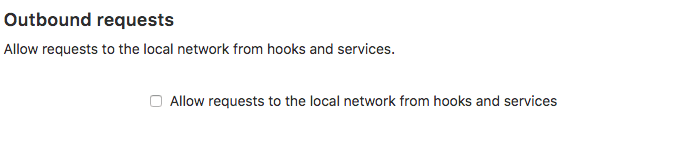
\includegraphics[width=13cm]{img/webhook_gitlab_setup.png}\\
			\caption[Webhook, GitLab]{Configurazione webhook con destinazione in rete locale}
		\end{figure}
		Ulteriori informazioni al riguardo possono essere trovate nella pagina\footnote{\url{https://docs.gitlab.com/ee/security/webhooks.html}} relativa a questo argomento sulla parte del sito relativa alla documentazione di GitLab.


		\paragraph{Configurazione destinazione}
		Successivamente si può aggiungere un indirizzo di destinazione di un webhook al progetto andando su \texttt{Settings > Integrations}.\\
		Da qui si possono selezionare gli eventi di interessi per i quali i webhook verranno attivati (attenzione: \progetto~non supporta tutti gli eventi, solamente quelli richiesti da \II).\\
		Nel campo relativo all'URL di destinazione inserire l'indirizzo, con relativa porta (nel nostro caso quella specificata nella Tabella 2), su cui il Producer GitLab è in ascolto.

		\paragraph{Eventi supportati}
		Per GitLab gli eventi supportati sono:
		\begin{itemize}
			\item Push events
			\item Comments
			\item Issues events
		\end{itemize}


---


	%TODO RIVEDERE
	La configurazione dei consumer e dei producer sono composte da file json contenti informazioni come ad esempio la mail di invio e la password relativa utilizzate per accedere al server mail.
	Queste possono essere modificate in modo tale da rispecchiare la configurazione che si vuole usare.

\subsection{Servizi aggiuntivi}
Aggiungere servizio necessario per il monitoraggio di kafka
Altri servizi per monitoraggio ?
